%!TEX root = draft.tex

\section{Empirical Analysis}
\label{sec:Analysis}

In this section, we begin by describing six large-scale network datasets that we use in our
analysis and experiments. Then, we
describe key factors that impact edge formation and analyze global structural
properties of real-world networks. Finally, we briefly discuss insights from
empirical studies in sociology and common assumptions in network modeling.

\subsection{Datasets}
\label{sec:Datasets}

We consider six citation networks of different scales (size, time) from diverse
sources: research articles, utility patents and judicial cases. We list the
summary statistics and global network properties of these datasets in~\Cref{table:datasets}.
Three of the six datasets are attributed networks; that is, each node has a categorical attribute value.

We focus on citation networks for two reasons. First, since nodes in citation networks form
all outgoing edges to existing nodes at the time of joining the network,
citation networks provide a clean basis to study edge formation mechanisms in
attributed social networks. Second, citation network span long periods of time (e.g.,
the \texttt{USSC} judicial citation network span several hundred years).
Consequently, identifying local edge formation processes that successfully model
growth for this duration is non-trivial.
Next, we study the structural and content properties of these networks.

% Now, we briefly describe the datasets considered in this paper.
% \Cref{table:datasets} provides summary statistics of the following networks:
% \begin{enumerate}
%     % (V,E) = (22049, 138871), used (V,E): 18665 115358
%     \item{\textbf{Association of Computational Linguistics}} (\texttt{ACL}) \cite{acldata} is an attributed academic citation network
%     that consists of papers published in ACL conferences, journals and workshops.
%     The attribute value of each paper is the name of the venue where it was published.
%
%     % (V,E) = (22049, 138871), used (V,E): 18665 115358
%     % \item{\textbf{Python Package Index}} (\texttt{PYPI}) \footnote{http://web.stanford.edu/class/cs224w/resources.html} is an attributed dependency graph of Python
%     % software packages. Each software package is associated with a category.
%
%     % entire dataset used
%     \item{\textbf{U.S. Supreme Court Cases}} (\texttt{USSC}) \cite{fowler2008authority} is a judicial citation network of
%     U.S. Supreme Court cases. There is an edge from case $i$ to case $j$ if and only if case $i$ cites case $j$ in its majority opinion.
%
%     % used: (V,E) = (30,558, 347,228) after removing nodes w. missing time data
%     \item{\textbf{ArXiv HEP-PH}} (\texttt{HEP-PH}) \cite{gehrke2003overview} is an academic citation network of HEP-PH (high energy
%     physics phenomenology) papers in the ArXiv e-print.
%
%     % used: (V,E) = (556661, 6647769) after removing nodes w. missing time + categorial data
%     \item{\textbf{APS Journals}} (\texttt{APS}) is an attributed academic citation network maintained by
%     the American Physical Society (\texttt{APS}).
%     The attribute value of each paper is the \texttt{APS} journal in which it was published.
%
%     % used: (V,E) = (2047881, 10088564) after removing nodes w. missing time + categorical data
%     \item{\textbf{U.S Utility Patents}} (\texttt{Patents}) \cite{leskovec2005graphs} is an attributed citation network of U.S. utility patents maintained by
%     the National Bureau of Economic Research (NBER).
%     The attribute value of each patent is an NBER patent category.
%
%     % used: (V,E) = (5987642, 45028807) after removing nodes w. missing time data
%     \item{\textbf{Semantic Scholar}} (\texttt{Semantic}) \cite{ammar} is an academic citation network of
%     Computer Science and Neuroscience papers, released in June 2017 by Semantic Scholar.
% \end{enumerate}

% in \cref{subsec:factors} and empirically
% validate the effectiveness of the proposed model using these network datasets in~\Cref{sec:Experiments}.
%
% In this section, we outlined the citation network datasets that we use in our analysis and experiments.
% Next, we discuss common factors that affect edge formation mechanisms and identify common global structural
% properties of real networks.


\subsection{Observations from Network Data}
\label{subsec:factors}

% Factors that influence edge formation at the nodal level have a cumulative
% effect on global structural properties of real-world networks.
Compact
statistical descriptors of global network properties ~\cite{newman2010networks}
such as degree distribution, local clustering, and attribute assortativity
quantify the extent to which local edge formation phenomena shape global network
structure.

\textbf{Heavy tailed degree distribution:} All networks in~\Cref{table:netstats} exhibit heavy tailed degree distributions. These
distributions can emerge from the well-known preferential attachment process~\cite{simon1955class,barabasi1999emergence}, where incoming nodes connect with nodes in proportion to their degree. As a result, initial differences in node
degree get reinforced over time, giving rise to heavy
tailed degree distributions.
% (also known as the ``rich get richer'' effect) in citation networks; It also implies that most papers receive zero or a few
% citations, but a small but significant percent of the nodes turn into popular
% hubs that receive many citations.
Log-normal fits, with parameters listed in~\Cref{table:netstats}, well describe the in-degree
distribution of all network datasets, consistent Broido and Clauset's~\cite{broido2018scale} observation that real-world networks with truly power law
degree distributions are rare.
% Our model explains the emergence of heavy tailed in-degree distributions through a \textit{local} process that adjusts bias towards linking to well-connected nodes

\begin{figure}[H]
 \vspace{-10pt}
 \centering
 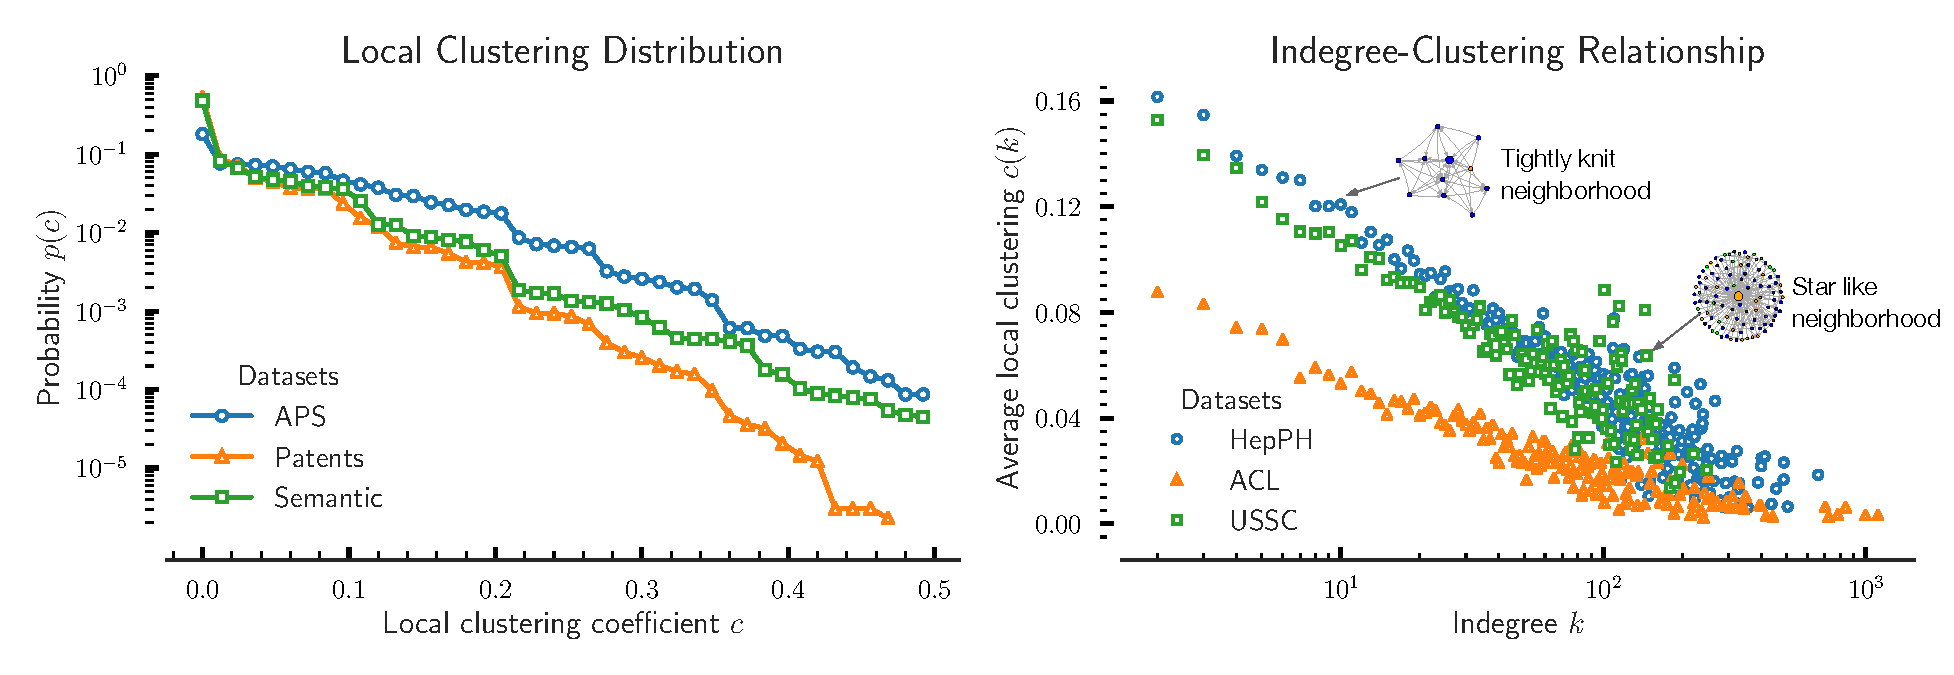
\includegraphics[width=\columnwidth]{cc_analysis3f}
 \caption{
    Local clustering in real-world networks have common characteristics:
    skewed local clustering distribution (left subplot) and a negatively correlated
    relationship between in-degree and average local clustering (right subplot).
 }
 \label{fig:cc_dc}
 \vspace{-10pt}
\end{figure}

\textbf{High Local Clustering:} Real-world networks tend to exhibit high average local clustering (\texttt{LCC}), as shown in~\Cref{table:netstats}. We can explain local clustering due to the phenomena of triadic closure~\cite{simmel1950sociology,
newman2001clustering}, where nodes with common neighbor(s) have an increased
likelihood of forming a connection.
% Empirical studies
% \cite{kossinets2006empirical} show that the probability of edge formation
% increases with the number of common neighbors.
The local clustering coefficient of a node measures the prevalence of triadic closure in its neighborhood. It is the probability that two randomly chosen neighbors of the node $i$ are connected. In directed networks, the neighborhood of a node $i$ can refer to the
set of nodes that link to $i$, set of nodes that $i$ links to or the union of
both sets. We define the neighborhood to be the set of all nodes that link to
node $i$.  However, average local clustering is not a
representative statistic of the {skewed} local clustering distributions
shown in~\Cref{fig:cc_dc}. Furthermore, real-world networks exhibit a negative
correlation between node in-degree  and local clustering. In~\Cref{fig:cc_dc}, we
also observe that the average local clustering  decreases as in-degree increases.
That is, low in-degree nodes have small, tightly knit neighborhoods and high
in-degree nodes tend have large, star-shaped neighborhoods.

% We propose a model
% that explains how clustering in real-world networks can arise from local processes
% of exploration \& link formation.


% Homophily and Assortativity
\textbf{Homophily:}
Attributed networks exhibit homophily~\cite{mcpherson2001birds}, the phenomenon where similar nodes are more likely
to be connected than dissimilar nodes. The assortativity coefficient
~\cite{newman2002assortative} $r \in [-1, 1]$,
% defined as the ratio between the observed modularity and
% the maximum possible modularity with respect to set of attribute values $B=\{b_1...b_l\}$,
quantifies the level of homophily in an attributed network. Intuitively, it
compares the observed fraction of edges between nodes with the same attribute
value to the expected fraction of edges between nodes with same attribute value
if the edges were rewired randomly.
Attributed networks \texttt{ACL}, \texttt{APS} and \texttt{Patents} exhibit
varying level of homophily, as shown in~\Cref{fig:mixing}, with assortativity
coefficient ranging from $0.07$ to $0.72$.
The magnitude of the attribute assortativity
signifies the extent to which attribute similarity influences edge formation.

% We embed attribute based preferences at the local level lead to generate networks
% with varying attribute mixing patterns.

\begin{figure}
 \centering
 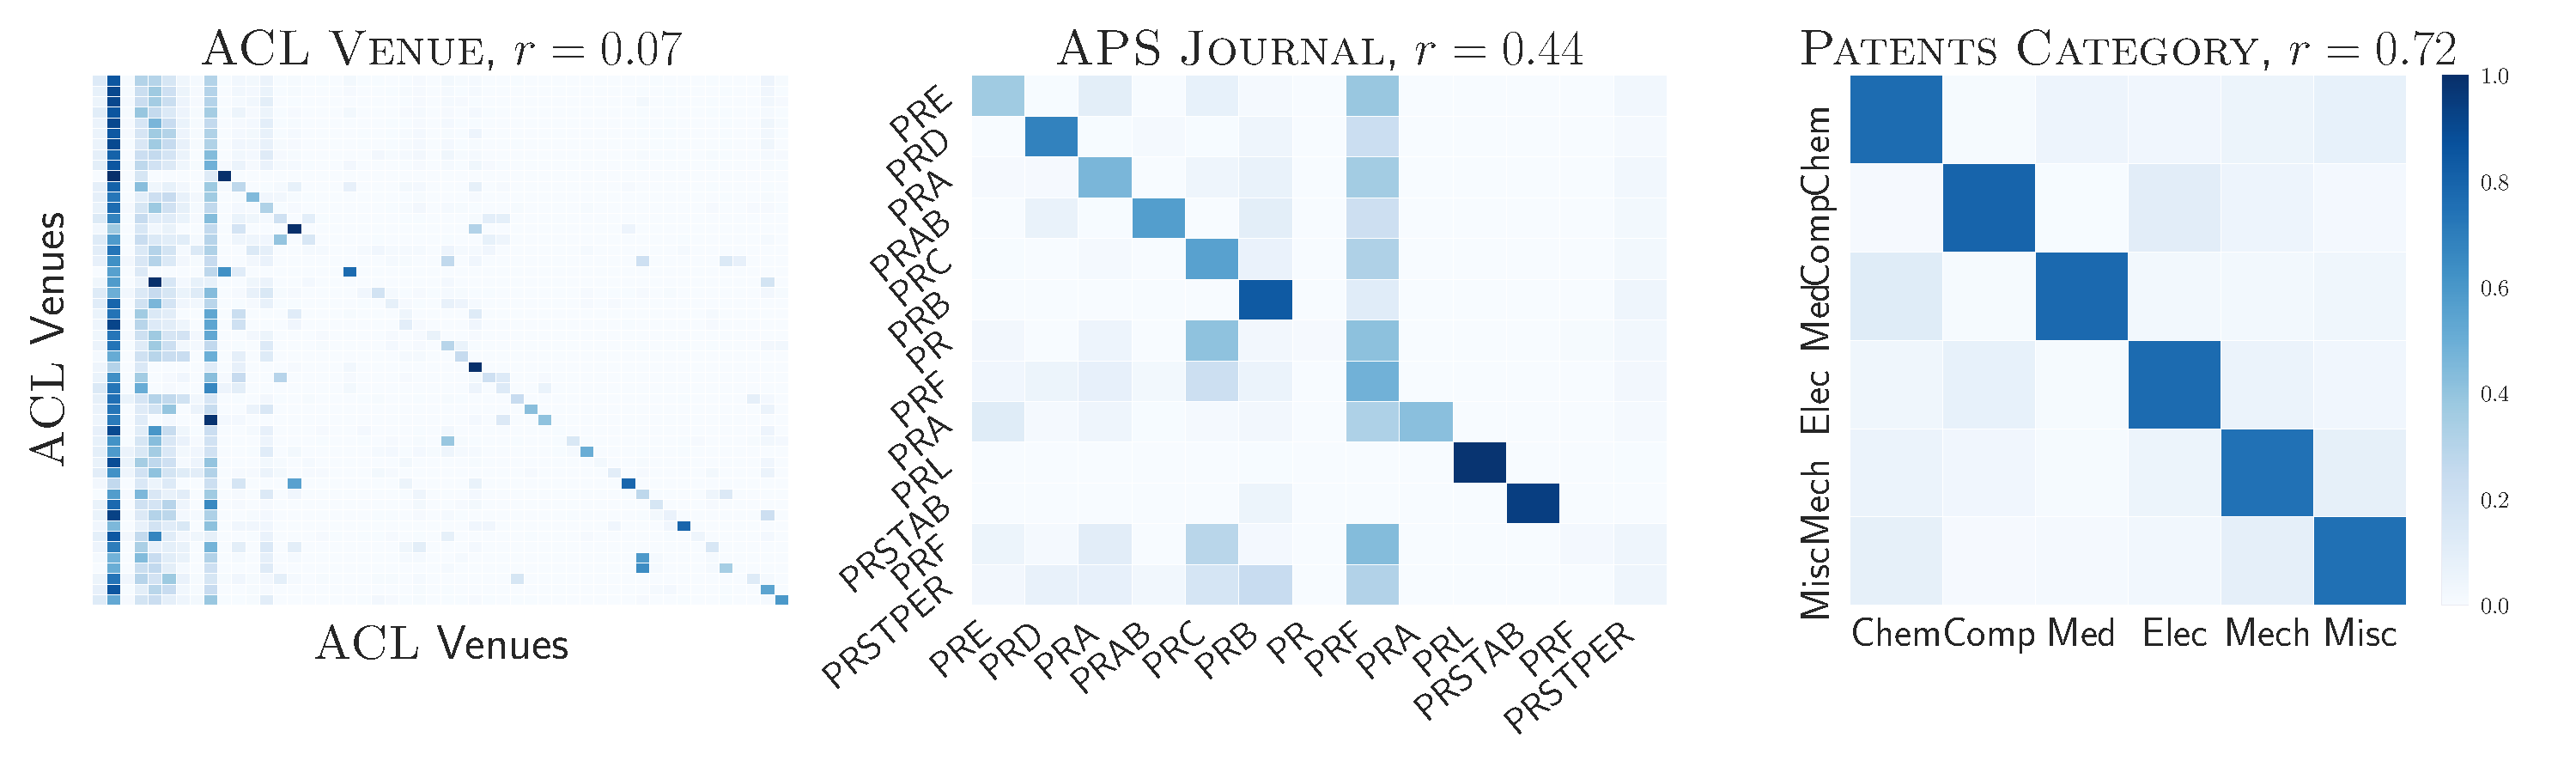
\includegraphics[width=\columnwidth]{homophily}
 \caption{
    Attributed networks exhibit varying levels of homophily. The subplots
    illustrate the mixing patterns in \texttt{ACL}, \texttt{APS} and \texttt{Patents}
    w.r.t. attributes \texttt{Venue} ($r=0.07$), \texttt{Journal} ($r=0.44$) and
    \texttt{Category} ($r=0.72$) respectively.
 }
 \label{fig:mixing}
 \vspace{-15pt}
\end{figure}

\textbf{Increasing Out-degree over Time:}
The out-degree of nodes that join real-world networks tends to increase
as functions of network size and time. This phenomenon densifies networks and shrinks their
diameter over time. Densification tends to exhibit a power law relationship
~\cite{leskovec2005graphs} between the number of edges $e(t)$ and nodes $n(t)$ at time $t$: $e(t) \propto n(t)^{\alpha}$.~\Cref{table:netstats} lists the densification power law (\texttt{DPL}) exponent $\alpha$ of the network datasets.

To summarize, citation networks tend to be homophilic networks that undergo
accelerated network growth and exhibit regularities in structural properties:
heavy tailed in-degree distribution, skewed local clustering distribution,
negatively correlated degree-clustering relationship, and varying attribute
mixing patterns.

% In our proposed model, we increase the outdegree of incoming nodes at a linear or superlinear rate to account for the accelerated network growth observed in real networks.

% To summarize, factors such as preferential attachment, triadic closure and homophily not only effect how individuals form connections at the local level but also explain regularities arise in global structural properties of real-world networks. Next, we discuss empirical studies from sociology that examine network formation and decision making.

\subsection{Insights from Sociological Studies}

Sociological studies on network formation seek to explain
how individuals form edges in real-world networks.

\textbf{Interplay of Triadic Closure and Homophily:} Empirical studies~\cite{35626,block2014multidimensional} that investigate
the interplay between triadic closure and homophily in evolving networks
indicate that \textit{both} structural proximity and homophily are statistically
significant factors that simultaneously influence edge formation. While homophilic preferences~\cite{mcpherson2001birds} induce edges between similar nodes, structural factors (e.g., network distance) act as constraints that restrict edge formation to structurally proximate nodes (e.g. friend of a friend).

\textbf{Bounded Rationality:} Extensive work~\cite{simon1972theories,gigerenzer1996reasoning,lipman1995information}
on individual decision making indicates that individuals are boundedly
rational actors. That is, individuals make decisions under constraints of limited information, cognitive capacity and time. This implies that individuals that join networks employ simple rules to form edges under constraints of limited information and partial network access. For example, a researcher cites academic papers without knowledge of, or access
to, the entire literature in her field.

Current preferential attachment and fitness-based models
\cite{dorogovtsev2000structure,kim2017effect,singh2017relay,barabasi1999emergence} make two assumptions that are at variance with these findings in the Social Sciences. First, by assuming that successive edge formations are independent, these models disregard the effect of triadic closure and structural proximity. Second, these models implicitly require incoming nodes to have complete network access (e.g., be able to connect to any node) or explicit knowledge of one or more properties (e.g., fitness, degree) of every node in the network. For example, a preferential attachment model, by making connections in proportion to degree, requires non-local information: the degree distribution of the entire network.

To summarize, insights from the Social Sciences suggest that edge formation in real-world networks is biased towards nodes that are similar, proximate or well-connected and that
these edges are made under constraints of limited information and network access.
The global properties described in~\Cref{subsec:factors} are modulated by the presence of
resource constrained edge formation decisions.

Next, we propose a growth model that explains how local processes of
edge formation can lead to the emergence of well-defined global structural and
attribute properties observed in real-world networks.

% citation networks tend to be homophilic networks that
% undergo accelerated network growth and exhibit regularities in structural
% properties: heavy tailed in-degree distribution, skewed local clustering distribution, negatively correlated degree-clustering relationship and varying attribute mixing patterns. These global properties are modulated by the presence of resource constrained edge formation decisions.


% and global structural properties can be better understood by studying network snapshots at different stages of the growth process.


% datasets include the time (e.g., publication year of academic papers) at which nodes join the network. As a result, local edge formation processes and global structural properties can be better understood by studying network snapshots at different stages of the growth process. Third, the citation networks are large networks that tend to have one or more nodal attributes (e.g. category of patents)
% and span multiple decades. As a result, the structural and content properties of the citation
% networks considered are well-defined.

% Nodes do
% not form or delete edges at a later time. This allows us to analyze
% the edge formation mechanisms of new nodes that join the network form edges.
% % Other edge dynamics such as edge deletion and addition of edges between existing
% % nodes are important and we plan to investigate them at a later time.
% Second, citation network datasets include the time (e.g., publication year of academic
% papers) at which nodes join the network. As a result, local edge formation
% processes and global structural properties can be better understood by studying
% network snapshots at different stages of the growth process. Third, the citation
% networks are large networks that tend to have one or more nodal attributes (e.g. category of patents)
% and span multiple decades. As a result, the structural and content properties of the citation
% networks considered are well-defined.

% \begin{table}[b]
%  \center
%  {
%   \begin{tabular}[c]{lrrrr} \toprule
%   Network Dataset &  \texttt{LN} $(\mu, \sigma)$ & \texttt{DPL} $\alpha$       &  Avg. ${\texttt{LCC}}$  & \texttt{AA} $r$   \\ \midrule
%   \texttt{USSC}     &   (1.19, 1.18) & 2.32     & 0.12    & -     \\
%   \texttt{HEP-PH}   &   (1.32, 1.41) & 1.67     & 0.12    & -     \\
%   \texttt{Semantic} &   (1.78, 0.96)  & 1.58     & 0.06    & -     \\   \midrule
%   \texttt{ACL}      &   (1.93, 1.38)  & 1.43     & 0.07    & 0.07     \\
%   \texttt{APS}      &   (1.62, 1.20)  & 1.26     & 0.11    & 0.44     \\
%   \texttt{Patents}  &   (1.10, 1.01)   & 1.94     & 0.04    & 0.72    \\
%   % \texttt{PYPI}         & 1.208     & 0.0524    & 0.692   & a\\
%    \bottomrule
%   \end{tabular}
%   \vspace{1mm}
%   \caption{Global network properties: lognormal (\texttt{LN}) in-degree distribution mean and standard deviation $(\mu, \sigma)$,
%   densification power law (\texttt{DPL}) exponent $\alpha$, average local clustering coefficient (${\texttt{LCC}}$)
%   and attribute assortativity (\texttt{AA}) coefficient of six network datasets.}
%   \label{table:netstats}
%  }
% \end{table}

